% !TeX root = ../NotesOnLQG.tex

\chapter{正则圈量子引力的运动学:代数及其表示}

	在前面的讨论中,通过将 Ashtekar 联络作为基本位型变量,我们建立了一个经典的哈密顿体系。在上一节中我们建立了约束系统量子化的流程,现在进行量子化,得到正则圈量子引力。

	\section{\texorpdfstring{Holonomy-Flux 代数 $\staralgebra{B}$}{Holonomy-Flux 代数 B}}

		经典位型空间选为 $\spc$ 所有 $\su{2}$ 值联络的集合 $\configurationspace{A}$。我们假定丛是平凡的,于是经典位型空间也即所有 $\su{2}$ 值一形式的集合。%按照量子力学的量子化流程,应当考虑以某种测度下的 $L^2(\configurationspace{A})$ 作为希尔伯特空间。然而,同通常的量子场论的情况一样,$\configurationspace{A}$ 是无穷维的流形,这给积分测度的定义带来麻烦,合理的积分测度常常不存在。一种解决办法是将经典位型空间稍加修改,得到一个可以定义积分测度的空间,称为量子位型空间。对于标量场的讨论可参见 \cite{Ashtekar2004}。
		如前所述,我们需要考虑 $f\in C^\infty(\configurationspace{A})$。为此最好找到一族 smeared 联络,然后考虑这些 smeared 量的函数。由于 $\tensor{A}{^i_a}$ 是一形式,它可以背景独立地在曲线上积分。根据在 杨-米尔斯 理论中已有的经验,可以考虑用 \emph{和乐}(holonomy)smear 联络:
		\begin{Definition}[Holonomy]
			给定联络 $\tensor{A}{^i_a}$ 和某曲线 $c$,考虑以下平移方程
			\begin{equation}
				\left\{
					\begin{gathered}
						\dv{t}h_c(A,t) = - \left( \tensor{A}{^i_a}(c(t)) \tensor{\dot{c}}{^a}(t) \tensor{\tau}{_i} \right) h_c(A,t),\\
						h_c(A,0) = \II \qc t\in\left[ 0,1 \right]
					\end{gathered}
				\right.
			\end{equation}
			其中 $\tensor{\dot{c}}{^a}$ 是 $c$ 的切矢,$\II$ 是 $\SU{2}$ 的单位元,则定义和乐 $h_c(A) \definedby h_c(A,1)$。
		\end{Definition}
		%对于空间流形 $\spc$,我们先通过“离散化”来将要考虑的自由度降为有限维。具体来说,我们选取 $\spc$ 上任意的包含有限条边的有向图 $\Gamma$,设它包含 $L$ 条有向边,记为 $\left\{ e_1, \cdots, e_L \right\}$,则联络一形式可自然在这些边上“积分”得到\emph{和乐}(holonomy)$h_{e_1}(A), \cdots, h_{e_L}(A)$,这便只有 $L$ 个自由度,要恢复所有自由度,则考虑所有可能的图即可。具体来说,和乐的定义为联络一形式所决定的沿曲线的平移,给定联络 $\tensor{A}{^i_a}$ 和某曲线 $c$,考虑以下平移方程
		% \begin{equation}
		% 	\left\{
		% 		\begin{gathered}
		% 			\dv{t}h_c(A,t) = - \left( \tensor{A}{^i_a}(c(t)) \tensor{\dot{c}}{^a}(t) \tensor{\sigma}{_i} \right) h_c(A,t),\\
		% 			h_c(A,0) = \II \qc t\in\left[ 0,1 \right]
		% 		\end{gathered}
		% 	\right.
		% \end{equation}
		% 其中 $\tensor{\dot{c}}{^a}$ 是 $c$ 的切矢,$\II$ 是 $\SU{2}$ 的单位元,则定义和乐 $h_c(A) \definedby h_c(A,1)$。
		可以证明和乐具有以下表达式
		\begin{equation}
			h_c(A) = \pathorder \exp(-\int_c \tensor{A}{^i_a} \tensor{\tau}{_i}),\label{eq-holonomy}
		\end{equation}
		其中 $\pathorder$ 表示 path-ordering,该表达式实际是一个级数\cite{Baez1994,Nakahara2003}。

		\nomenclature{$\configurationspace{A}$}{经典位型空间,$\su{2}$值联络的集合}
		\nomenclature{$h_c(A)$}{联络$A$沿 $c$ 的 holonomy}

		容易验证,在规范变换 $g$ 和空间微分同胚变换 $\phi$ 下,和乐的变换为
		\begin{equation}
			h_c(A) \mapsto g(t(c))^{-1} h_c(A) g(s(c)) \qc h_c(A) \mapsto h_{\varphi\circ c}(A),
		\end{equation}
		其形式比较简单,便于构造规范不变量,这是采用和乐而不是形如 $\int_{\spc} \tensor{f}{^a_i} \tensor{A}{^i_a}$ 的表达式作为 smeared 联络的原因。但也应注意到,只在一维上smear联络的后果是 $h_c(A)$ 对 $\tensor{A}{^i_a}$ 的泛函导数包含分布,它实际上并不是场 $\tensor{A}{^i_a}$ 的光滑函数,而不像 $\int_{\spc} \tensor{f}{^a_i} \tensor{A}{^i_a}$ 那样。好在,只需要尽量避免 $\staralgebra{B}$ 中出现分布即可。为此需在至少二维的对象上 smear 动量。考虑动量 $\tensor{\tilde{P}}{^a_i}$ 的对偶 $\tensor[^*]{P}{^i_a_b} \definedby \tensor{\tilde{P}}{^c_j} \tensor{\nvol}{_a_b_c} \tensor{\delta}{^i^j}$,其中 $\tensor{\nvol}{_a_b_c} = \tensor{\vol}{_a_b_c}/\sqrt{h}$ 是 $\spc$ 上的 Levi-Civita 张量密度,则它可在二维面 $S$ 上积分得到 \emph{flux}
		\begin{equation}
			\tensor{P}{_i}(S) \definedby \int_S \tensor[^*]{P}{^i_a_b},
		\end{equation}
		并记 $P(S) = \tensor{\delta}{^i_j} \tensor{P}{_i}(S) \tensor{\tau}{_j}$,则 $P(S)$ 在规范变换 $g$ 和空间微分同胚变换 $\phi$ 下具有以下变换
		\begin{equation}
			P(S) \mapsto \int_S \Ad{g}\left( \tensor[^*]{P}{^i_a_b} \right) \qc P(S) \mapsto P(\phi^{-1}(S)),
		\end{equation}
		可以看到微分同胚变换依然很简单,但规范变换稍复杂。尽管如此,还是可以用 $P(S)$ 构造规范不变的量,例如以后将构造的面积泛函和面积算符。

		\nomenclature{$\tensor{P}{_i}(S)$}{面$S$上的flux}

		接下来定义 \emph{holonomy-flux algebra}。可以证明若两个光滑联络对任意曲线的和乐相同,则这两个联络相同,故和乐可看作 $\configurationspace{A}$ 上的“坐标”。于是我们先考虑 $\configurationspace{A}$ 上只依赖于有限个“坐标”的函数 $f$,即考虑给定有限个光滑曲线 $\left\{ c_1, \cdots, c_n \right\}$,具有 $f(A) = f_\gamma(h_{c_1}(A),\cdots,h_{c_n}(A))$ 形式的函数,其中 $f_\gamma$ 是 $\SU{2}^n$ 上的函数。稍具体一些来说,我们取一个图 $\gamma$,其中只包含有限个边(edge)和顶点(vertex),且边至多只在两端相交。边和顶点的集合分别记为 $E(\gamma)$ 和 $V(\gamma)$。接下来给出\emph{柱函数}(cylindrical function)的粗略定义:
		\begin{Definition}
			对图 $\gamma$ 定义映射
			\begin{equation}
				p_\gamma \colon \configurationspace{A} \rightarrow {\SU{2}}^{\card{E(\gamma)}} \qc
				\tensor{A}{^i_a} \mapsto \left\{ h_e(A) \right\}_{e \in E(\gamma)},\label{eq-p_gamma}
			\end{equation}
			则 $f\colon \configurationspace{A} \rightarrow \mathbb{C}$ 称为是相对于图 $\gamma$ 的 $k$ 阶连续可微的柱函数,当且仅当存在 $k$ 阶连续可微的 $f_\gamma \colon {\SU{2}}^{\card{E(\gamma)}} \rightarrow \mathbb{C}$,使得 $f=f_\gamma \circ p_\gamma$。将 $\gamma$ 上 $k$ 阶连续可微的柱函数的集合记为 $\Cyl_\gamma^k$,并定义 $\Cyl^k = \left\{ f \,\middle\vert\, \exists \gamma \;\text{s.t.}\; f\in \Cyl_\gamma^k \right\}$。
		\end{Definition}
		李代数 $\staralgebra{B}$ 将基于用 $\Cyl^\infty$ 作为 $C^\infty(\configurationspace{A})$。还需计算 $\left\{ p, f \right\}$,在这里即 $\left\{ P_i(S), f \right\}$,其中 存在 $\gamma$ 使得 $f\in \Cyl_\gamma^\infty$,首先使用链式法则
		\begin{equation}
			\left\{ P_i(S), f \right\}(A) = \sum_{l=1}^{\card{E(\gamma)}} \eval{\pdv{f_\gamma\left( h_1, \cdots , h_{\card{E(\gamma)}} \right)}{\tensor{(h_l)}{_m_n}}}_{h_j=h_{e_j}(A),\forall j} \left\{ P_i(S), \tensor{(h_{e_l})}{_m_n} \right\}(A),
		\end{equation}
		对于 holonomy 和 flux 的泊松括号,这里直接给出结果,可参考 \cite{Thiemann2007,Thiemann0210094}。
		\begin{Property}
			设有定向的面 $S$ 和曲线 $e$,且 $e$ 要么包含于 $S$,要么至多与 $S$ 相交于顶点(总可以分割 $e$ 使每一段都满足此条件)。则
			\begin{equation}
				\left\{ P_i(S), h_e(A) \right\} = \frac{\kappa(S,e)}{2} \times
				\begin{cases}
					h_e(A) \tensor{\tau}{_i}, &\qif* S\cap e = s(e),\\
					- \tensor{\tau}{_i} h_e(A), &\qif* S \cap e = t(e),
				\end{cases}
			\end{equation}
			其中
			\begin{equation}
				\kappa(S,e) \definedby
				\begin{cases}
					0, &\qif* S\cap e = \emptyset \qor e,\\
					+1, &\qif* S\cap e = \{p\} \qand \text{$e$ 在 $S$ 上方},\\
					-1, &\qif* S\cap e = \{p\} \qand \text{$e$ 在 $S$ 下方},
				\end{cases}
			\end{equation}
			$s(e),t(e)$ 分别指 $e$ 的起点和终点,“上方”指 $S$ 的法余矢 $\tensor{n}{_a}$ 的一侧。
		\end{Property}
		于是可以得到泊松括号
		\begin{equation}
			\begin{split}
				\left\{ P_i(S), f \right\}(A) ={}& \frac{1}{2} \sum_{l:e_l\cap S = s(e_l)} \eval{\pdv{f_\gamma\left( h_1, \cdots , h_{\card{E(\gamma)}} \right)}{\tensor{(h_l)}{_m_n}}}_{h_j=h_{e_j}(A),\forall j} \kappa(S,e_l) (h_{e_l}(A) \tensor{\tau}{_i})_{m,n}\\
				&-\frac{1}{2} \sum_{l:e_l\cap S = t(e_l)} \eval{\pdv{f_\gamma\left( h_1, \cdots , h_{\card{E(\gamma)}} \right)}{\tensor{(h_l)}{_m_n}}}_{h_j=h_{e_j}(A),\forall j} \kappa(S,e_l) (\tensor{\tau}{_i} h_{e_l}(A))_{m,n}\\
				={}& \frac{1}{2} \sum_{l:e_l\cap S = s(e_l)} \kappa(S,e_l) L_i^{(e_l)}f_\gamma(\left\{ h_e(A) \right\})\\
				&+ \frac{1}{2} \sum_{l:e_l\cap S = t(e_l)} \kappa(S,e_l) R_i^{(e_l)}f_\gamma(\left\{ h_e(A) \right\}),\label{eq-flux_function_algebra}
			\end{split}
		\end{equation}
		其中
		\begin{equation}
			\begin{gathered}
				L_i^{(e_l)} f_\gamma\left( h_1,\cdots,h_{\card{E(\gamma)}} \right) \definedby \eval{\dv{t}}_{t=0} f_\gamma \left( h_1,\cdots,h_{e_l} \e{t \tensor{\tau}{_i}},\cdots,h_{\card{E(\gamma)}} \right),\\
				R_i^{(e_l)} f_\gamma\left( h_1,\cdots,h_{\card{E(\gamma)}} \right) \definedby \eval{\dv{t}}_{t=0} f_\gamma \left( h_1,\cdots,\e{-t \tensor{\tau}{_i}} h_{e_l},\cdots,h_{\card{E(\gamma)}} \right)\label{eq-invariance_vector_field}
			\end{gathered}
		\end{equation}
		是 $\SU{2}^{\card{E(\gamma)}}$ 上的左不变矢量场和右不变矢量场。

		\nomenclature{$f_\gamma$}{图 $\gamma$ 上的柱函数}
		\nomenclature{$E(\gamma)$}{图 $\gamma$ 的边的集合}
		\nomenclature{$V(\gamma)$}{图 $\gamma$ 的顶点的集合}
		\nomenclature{$\Cyl_\gamma^k$}{图 $\gamma$ 上 $k$阶可微的柱函数的集合}
		\nomenclature{$\Cyl^k$}{$k$阶可微的柱函数的集合}
		\nomenclature{$L_i,R_i$}{$\SU{2}$上的左不变矢量场和右不变矢量场}

		定义 $\Cyl^\infty$ 上的矢量场 $v_S^i$
		\begin{equation}
			v_S^i(f) \definedby \left\{ P_i(S), f \right\},
		\end{equation}
		可定义 holonomy-flux algebra $\staralgebra{B}$ 为 $(f,v_S^i)$ 配以李括号
		\begin{equation*}
			\left[ \left( f, v \right), \left( f', v' \right) \right] \definedby \left( v(f') - v'(f), \left[ v, v' \right] \right)
		\end{equation*}
		生成的李 $*$-代数。

		\nomenclature{$\staralgebra{B}$}{holonomy-flux 代数}

	\section{\texorpdfstring{$\staralgebra{B}$ 的表示与kinematical 希尔伯特空间 $\Hkin$}{B 的表示与 kinematical 希尔伯特空间}}

		本部分介绍 $\staralgebra{B}$ 的不可约表示,若要求 flux 算符良定义且自伴,并要求表示是空间微分同胚不变的,则本节介绍的表示是唯一的。\cite{Thiemann2007}

		如前所述,$\Hkin$ 可选择为某种 $L^2(\bar{\configurationspace{A}},\mu)$,对此希尔伯特空间最简洁的描述是使用 $C^*$-代数的语言进行 GNS 构造\cite{Thiemann2007,Han2005},这里使用稍冗长但简单的几何描述来构造这个空间及 $\staralgebra{B}$ 在其上的表示。

		%经典位型空间选为 $\spc$ 上所有 $\su{2}$ 值联络的集合 $\configurationspace{A}$。我们假定丛是平凡的,于是经典位型空间也即所有 $\su{2}$ 值一形式的集合。按照量子力学的量子化流程,应当考虑以某种测度下的 $L^2(\configurationspace{A})$ 作为希尔伯特空间。然而,同通常的量子场论的情况一样,$\configurationspace{A}$ 是无穷维的流形,这给积分测度的定义带来麻烦,合理的积分测度常常不存在。一种解决办法是将经典位型空间稍加修改,得到一个可以定义积分测度的空间,称为量子位型空间。对于标量场的讨论可参见 \cite{Ashtekar2004},以下我们介绍该方法用于量子引力的结果。

		% 对于空间流形 $\spc$,我们先通过“离散化”来将要考虑的自由度降为有限维。具体来说,我们选取 $\spc$ 上任意的包含有限条边的有向图 $\Gamma$,设它包含 $L$ 条有向边,记为 $\left\{ e_1, \cdots, e_L \right\}$,则联络一形式可自然在这些边上“积分”得到\emph{holonomy}(holonomy)$h_{e_1}(A), \cdots, h_{e_L}(A)$,这便只有 $L$ 个自由度,要恢复所有自由度,则考虑所有可能的图即可。具体来说,holonomy的定义为联络一形式所决定的沿曲线的平移,给定联络 $\tensor{A}{^i_a}$ 和某曲线 $c$,考虑以下平移方程
		% \begin{equation}
		% 	\left\{
		% 		\begin{gathered}
		% 			\dv{t}h_c(A,t) = - \left( \tensor{A}{^i_a}(c(t)) \tensor{\dot{c}}{^a}(t) \tensor{\sigma}{_i} \right) h_c(A,t),\\
		% 			h_c(A,0) = \II \qc t\in\left[ 0,1 \right]
		% 		\end{gathered}
		% 	\right.
		% \end{equation}
		% 其中 $\tensor{\dot{c}}{^a}$ 是 $c$ 的切矢,$\II$ 是 $\SU{2}$ 的单位元,则定义holonomy $h_c(A) \definedby h_c(A,1)$。可以证明holonomy具有以下表达式
		% \begin{equation}
		% 	h_c(A) = \pathorder \exp(-\int_c \tensor{A}{^i_a} \tensor{\sigma}{_i}),
		% \end{equation}
		% 其中 $\pathorder$ 表示 path-ordering,该表达式实际是一个级数,参见\cite{Baez1994,Nakahara2003}。

		% 容易验证,在规范变换和空间微分同胚变换下,holonomy的变换为
		% \begin{equation}
		% 	h_c(A) \mapsto g(t(c))^{-1} h_c(A) g(s(c)) \qc h_c(A) \mapsto h_{\varphi\circ c}(A),
		% \end{equation}
		% 其形式比较简单,这是采用holonomy而不是形如 $\int_{\spc} \tensor{f}{^a_i} \tensor{A}{^i_a}$ 的表达式作为 smeared 联络的原因。

		\subsection{\texorpdfstring{量子位型空间$\bar{\configurationspace{A}}$}{量子位型空间}}

			需要先约定几个定义,稍后将用到它们:
			\begin{Definition}
				\begin{enumerate}
					\item 现在开始所谈论的\emph{曲线}(curve)$c$ 无特殊说明时,是指一个映射 $c\colon \left[ 0,1 \right] \rightarrow \spc$,要满足连续、分段半解析且每段是一个正则嵌入\footnote{要求曲线分段为正则嵌入是为了避免每小段曲线的像自交或任意接近自己的情况出现。}。记$s(c)\definedby c(0)$,称为曲线 $c$ 的 source、$t(c)\definedby c(1)$ 称为曲线 $c$ 的 target。这样的曲线的集合记为 $\setofcurve$。
					\item 在 $\setofcurve$ 上如通常代数拓扑的定义方式定义乘法 $\circ$ 和逆:
					\begin{enumerate}
						\item 若 $t(c) = s(c')$,定义 $c'' = c' \circ c$ 为
						\begin{equation}
							c''(t) \definedby
							\begin{cases}
								c(2t), & t \in \left[ 0, \frac{1}{2} \right],\\
								c'(2t-1), & t \in \left[ \frac{1}{2}, 1 \right],
							\end{cases}
						\end{equation}
						\item $\forall c \in \setofcurve$,定义其逆为
						\begin{equation}
							c^{-1}(t) \definedby c(1-t) \qc t \in \left[ 0,1 \right].
						\end{equation}
					\end{enumerate}
					\item 定义道路(path) $p$ 为曲线的等价类,其中等价关系 $\sim$ 定义为 $c\sim c'$ 当且仅当通过以下三种操作
					\begin{enumerate}
						\item 重参数化,即选择满足 $f'>0$ 的满射 $f\colon \left[ 0,1 \right] \rightarrow \left[ 0,1 \right]$,执行操作 $c \mapsto c\circ f$;
						\item 将 $c$ 分为两段 $c = s_2 \circ s_1$,选择 $s_3$ 使得 $s(s_3) = t(s_1)$,执行操作 $c = s_2 \circ s_1 \mapsto s_2 \circ s_3^{-1} \circ s_3 \circ s_1$;
						\item 若将 $c$ 适当分为4段,能使 $c$ 具有形式 $c= s_2 \circ s_3^{-1} \circ s_3 \circ s_1$,执行操作 $c= s_2 \circ s_3^{-1} \circ s_3 \circ s_1 \mapsto s_2 \circ s_1$\footnote{注意运算 $\circ$ 并没有结合律,但由于允许重参数化,就并不影响这里所写的式子。}
					\end{enumerate}
					在有限步之内能将 $c$ 变换为 $c'$。道路的集合记为 $\setofpath = \setofcurve/ \sim$。
					\item 现在起所说的\emph{图}(graph)是指一些道路的集合,并且这些道路要被适当分段使得每段都有解析的表示,并互相至多在端点处相交。这些分段后的道路称为\emph{边}(edge)$e$,其集合记为 $E(\gamma)$;边的端点称为\emph{顶点}(vertex),其集合记为 $V(\gamma)$。所有图的集合记为 $\Gamma$。
				\end{enumerate}
			\end{Definition}

			\nomenclature{$\gamma$}{图}
			\nomenclature{$\Gamma$}{图的集合}

			\begin{Remark}
				\begin{enumerate}
					\item 容易验证,$\setofcurve$ 上的 $\circ$ 和 $(\cdot)^{-1}$ 两种运算可良定义在 $\setofpath$ 上,且这两种运算使得 $\setofpath$ 构成一个\emph{广群}(groupoid)。
					\item 在 $\Gamma$ 上定义关系 $\prec$ 为 $\gamma \prec \gamma'$ 当且仅当任取 $e\in E(\gamma)$,$e$ 可以写为 $E(\gamma')$ 中有限条边或其逆的乘积。$\Gamma$ 配以关系 $\prec$ 构成一个\emph{有向集}(directed set),即任取 $\gamma,\gamma' \in \Gamma$,存在 $\gamma'' \in \Gamma$ 使得 $\gamma \prec \gamma''$ 且 $\gamma' \prec \gamma''$。
				\end{enumerate}
			\end{Remark}

			由~\eqref{eq-holonomy} 容易证明,给定联络,holonomy满足下列性质:
			\begin{Property}
				设 $s(c_2) = t(c_1)$,则
				\begin{equation}
					h_{c_2}(A) h_{c_1}(A) = h_{c_2 \circ c_1}(A) \qc h_{c}(A)^{-1} = h_{c^{-1}}(A).
				\end{equation}
			\end{Property}
			这使得 holonomy 实际上是定义在道路上的,任取 $p\in \setofpath$,取其一个代表元 $c$,即 $p=[c]$,则可定义
			\begin{equation}
				h_p(A) \definedby h_c(A),
			\end{equation}
			与 $c$ 的选择无关。并且同样有
			\begin{equation}
				h_{p_2}(A) h_{p_1}(A) = h_{p_2 \circ p_1}(A) \qc h_{p}(A)^{-1} = h_{p^{-1}}(A),
			\end{equation}
			于是联络可被视为广群同态
			\begin{equation}
				A \colon \setofpath \rightarrow \SU{2} \qc p \mapsto h_p(A),
			\end{equation}
			于是这种观点提供了一种定义广义联络的方式:
			\begin{Definition}[量子位型空间]
				量子位型空间 $\bar{\configurationspace{A}}$ 定义为 $\bar{\configurationspace{A}} \definedby \Hom{\setofpath}{\SU{2}}$,即所有广群同态。这样,联络 $\tensor{A}{^i_a} \in \configurationspace{A}$ 和 holonomy $h_p(A)$ 被推广为 $A \in \bar{\configurationspace{A}}$ 和 $A(p)$。
			\end{Definition}
			广义联络是不需要连续的,即 $A(p)$ 在 $p$ 连续变形时可以不连续变化。

			\nomenclature{$\bar{\configurationspace{A}}$}{量子位型空间}

			% 正如将标量场 smear 后可自然考虑将广义函数包括进来一样,可以自然地向经典位型空间 $\configurationspace{A}$ 中添加“广义联络”,即满足holonomy的所有性质的映射 $A: e \mapsto h_e(A)$,得到 \emph{量子位型空间} $\bar{\configurationspace{A}}$,这样做的好处是量子位型空间上将存在平方可积的良好定义,细节可参见 \cite{Ashtekar2004,Han2005}。

			% 有了holonomy的概念后,考虑 $\bar{\configurationspace{A}}$ 上的函数中,只依赖 $h_{e_1}(A), \cdots, h_{e_L}(A)$ 这些量的那些,即形如
			% \begin{equation}
			% 	\psi_{(\Gamma,f)}(A) = f(h_{e_1}(A), \cdots, h_{e_L}(A))
			% \end{equation}
			% 的,其中 $f$ 是 ${\SU{2}}^L$ 上的平方可积复函数,这里平方可积指
			% \begin{equation}
			% 	\int_{\SU{2}^L} \left( \dd{\mu} \right)^L \abs{f}^2
			% \end{equation}
			% 有限,其中 ${\mu}$ 是 $\SU{2}$ 上的哈尔测度(Haar measure)。将形如 $\psi_{(\Gamma,f)}$ 的函数称为图 $\Gamma$ 上的 \emph{柱函数}(cylindrical function),将其集合记为 $\Cyl_\Gamma$。在其上存在一个自然的内积定义
			% \begin{equation}
			% 	\left\langle \psi_{(\Gamma,f)} , \psi_{(\Gamma,g)} \right\rangle \definedby \int_{\SU{2}^L} \left( \dd{\mu} \right)^L \overline{f}g,
			% \end{equation}
			% 于是 $\left( \Cyl_\Gamma, \left\langle \cdot, \cdot \right\rangle \right)$ 构成一个依赖于图 $\Gamma$ 定义的希尔伯特空间,记为 $\Hil_\Gamma$。要找出完整的希尔伯特空间,则需要考虑所有可能的图。

		\subsection{\texorpdfstring{$\bar{\configurationspace{A}}$ 上的拓扑}{量子位型空间上的拓扑}}

			为了给 $\bar{\configurationspace{A}}$ 定义测度,这里先定义其上的拓扑。注意到式~\eqref{eq-p_gamma} 中定义的映射 $p_\gamma \colon \configurationspace{A} \mapsto \SU{2}^{\card{E(\gamma)}}$ 完全可改为定义在 $\bar{\configurationspace{A}}$ 上,而 $\SU{2}^{\card{E(\gamma)}}$ 在它自带的流形拓扑下是紧致豪斯多夫拓扑空间,于是可考虑如下过程构造的拓扑\cite{Thiemann2007}。

			给定图 $\gamma \in \Gamma$,定义 $\bar{\configurationspace{A}}_\gamma \definedby \Hom{\gamma}{\SU{2}^{\card{E(\gamma)}}}$,这里 $\gamma$ 被视作 $\setofpath$ 的子广群。则映射
			\begin{equation}
				\bar{\configurationspace{A}}_\gamma \rightarrow \SU{2}^{\card{E(\gamma)}} \qc A_\gamma \mapsto \left\{ A_\gamma(e) \right\}_{e \in E(\gamma)}
			\end{equation}
			是 $\bar{\configurationspace{A}}_\gamma$ 到 $\SU{2}^{\card{E(\gamma)}}$ 的双射,可用来将 $\SU{2}^{\card{E(\gamma)}}$ 的拓扑结构拉回到 $\bar{\configurationspace{A}}_\gamma$ 上。为复原整个 $\bar{\configurationspace{A}}$,进一步定义
			\begin{equation}
				\bar{\configurationspace{A}}_{\infty} \definedby \bigtimes_{\gamma \in \Gamma} \bar{\configurationspace{A}}_\gamma,
			\end{equation}
			则 $\bar{\configurationspace{A}}_\infty$ 上的乘积拓扑,或称 Tychonoff 拓扑是紧致且豪斯多夫的\footnote{紧致见 Tychonoff 定理,豪斯多夫不难证明,可参见\cite{munkres2000topology}。}。但由 $A \in \bar{\configurationspace{A}}$ 所诱导的 $A|_{\gamma}$ 却不是互相独立的,因此集合 $\bar{\configurationspace{A}}_\infty$ 比 $\bar{\configurationspace{A}}$ 要“大”。例如图~\ref{figure-twogragh} 所示,$\gamma \prec \gamma'$,此时 $A_\gamma$ 和 $A_{\gamma'}$ 之间有约束 $A_\gamma(e_{12}) = A_{\gamma'}(e_{32}) A_{\gamma'}(e_{13})$,$\bar{\configurationspace{A}}_\infty$ 中不满足此约束的元素是无法与 $\bar{\configurationspace{A}}$ 中的广义联络对应的。
			\begin{figure}[htbp]
				\centering
				\begin{tikzpicture}[scale=0.8,]
					\node[below left] (v1) at (0,0) {$v_1$};
					\node[right] (v2) at (4,2) {$v_2$};
					\node[below right] (e12) at (2,0.8) {$e_{12}$};
					\draw[\myarrow] (0,0) -- (2.2,1.1);
					\draw (2,1) -- (4,2) -- (2,3) -- (0,0);
					\node (gamma) at (2,-1) {{\Large $\gamma$}};
				\end{tikzpicture}
				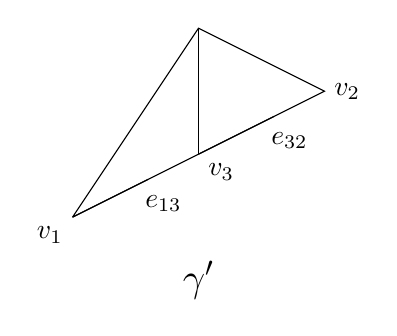
\begin{tikzpicture}[scale=0.8,]
					\node[below left] (v1) at (0,0) {$v_1$};
					\node[right] (v2) at (4,2) {$v_2$};
					\node[below right] (v3) at (2,1) {$v_3$};
					\node[below right] (e13) at (1,0.5) {$e_{13}$};
					\node[below right] (e32) at (3,1.5) {$e_{32}$};
					\draw[\myarrow] (0,0) -- (1.2,0.6);
					\draw[\myarrow] (2,1) -- (3.2,1.6);
					\draw (0,0) -- (4,2) -- (2,3) -- (0,0);
					\draw (2,1) -- (2,3);
					\node (gamma) at (2,-1) {{\Large $\gamma'$}};
				\end{tikzpicture}
				\caption{有偏序关系的图$\gamma$ 和 $\gamma'$}\label{figure-twogragh}
			\end{figure}

			为此,对于每一对图 $\gamma \prec \gamma'$ 引入图限制映射
			\begin{equation}
				p_{\gamma' \gamma} \colon \bar{\configurationspace{A}}_{\gamma'} \rightarrow \bar{\configurationspace{A}}_\gamma \qc h_{\gamma'} \mapsto \left.h_{\gamma'}\right|_{\gamma},
			\end{equation}
			它满足对于 $\gamma \prec \gamma' \prec \gamma''$ 有
			\begin{equation}
				p_{\gamma'' \gamma} = p_{\gamma' \gamma} \circ p_{\gamma'' \gamma'},
			\end{equation}
			则有
			\begin{equation}
				p_{\gamma' \gamma}\left( A_{\gamma'} \right) = A_\gamma,
			\end{equation}
			于是考虑如下定义
			\begin{Definition}
				投影系统(projective system)$\left\{ \bar{\configurationspace{A}}_\gamma, p_{\gamma' \gamma} \right\}$ 的\emph{投影极限}(projective limit)定义为 $\bar{\configurationspace{A}}_\infty$ 的一个子集
				\begin{equation}
					\varprojlim_{\gamma} \bar{\configurationspace{A}}_\gamma \definedby \left\{ {\left( h_\gamma \right)}_{\gamma \in \Gamma} \in \bar{\configurationspace{A}}_{\infty} \,\middle\vert\, p_{\gamma' \gamma}(h_{\gamma'}) = h_\gamma\qc \forall \gamma \prec \gamma' \right\}.
				\end{equation}
			\end{Definition}
			我们不加证明地列出以下结果:
			\begin{Property}
				\begin{enumerate}
					\item $p_{\gamma' \gamma}$ 都是连续满射;
					\item $\varprojlim_{\gamma} \bar{\configurationspace{A}}_\gamma$ 是 $\bar{\configurationspace{A}}_\infty$ 的闭子集,因而在子空间拓扑下也是紧致豪斯多夫空间;
					\item 映射
					\begin{equation}
						\Phi \colon \bar{\configurationspace{A}} \rightarrow \varprojlim_{\gamma} \bar{\configurationspace{A}}_\gamma \qc A \mapsto {\left( h_\gamma \definedby A|_\gamma \right)}_{\gamma \in \Gamma}
					\end{equation}
					是双射。
				\end{enumerate}
			\end{Property}
			至此,用 $\Phi$ 将 $\bar{\configurationspace{A}}$ 与 $\varprojlim_{\gamma} \bar{\configurationspace{A}}_\gamma$ 认同,即在 $\bar{\configurationspace{A}}$ 上定义了一个紧致豪斯多夫拓扑。

		\subsection{\texorpdfstring{$\bar{\configurationspace{A}}$上的测度}{量子位型空间上的测度}}

			上一节中为 $\bar{\configurationspace{A}}$ 定义的紧致豪斯多夫拓扑将对其上测度的定义起到很大帮助。本节定义 $\bar{\configurationspace{A}}$ 上的 Ashtekar-Lewandowski 测度,参见\cite{Ashtekar1994,Thiemann0210094,Thiemann2007}。

			考虑连续函数的集合 $C\left(\bar{\configurationspace{A}}\right)$,根据 Riesz-Markov-Kakutani 表示定理,由于 $\bar{\configurationspace{A}}$ 具有紧致豪斯多夫拓扑,其上的正则 Borel 测度 $\mu$ 与 $C\left(\bar{\configurationspace{A}}\right)$ 上的正定线性泛函 $\Lambda$ 通过下式一一对应
			\begin{equation}
				\Lambda\left(f\right) = \int_{\bar{\configurationspace{A}}} \dd{\mu} f \qc \forall f \in C\left(\bar{\configurationspace{A}}\right).
			\end{equation}
			注意到 $C\left(\bar{\configurationspace{A}}\right)$ 上可定义上确界范数 $\norm{f} \definedby \sup_{A \in \bar{\configurationspace{A}}} \abs{f(A)}$,可以检验 $C\left(\bar{\configurationspace{A}}\right)$ 构成 $C^*$-代数,则一个泛函分析中的标准结果是 $C\left(\bar{\configurationspace{A}}\right)$ 上的线性泛函自动是连续的,因而有界,且 $\norm{\Lambda} = \Lambda(1)$,故我们总可以选择 $\Lambda$ 使 $\Lambda(1)=1$,则 $\mu$ 是一个概率测度。

			为了明确定义一个 $\Lambda$,考察柱函数与 $C\left(\bar{\configurationspace{A}}\right)$ 的关系。这里重新定义一下 $\Cyl^k\left(\bar{\configurationspace{A}}\right)$ 以代替之前在 $\configurationspace{A}$ 上定义的 $\Cyl^k$。
			\begin{Definition}
				取两个 $k$ 阶可微的函数 $f_\gamma \in C^k\left(\bar{\configurationspace{A}}_\gamma\right)$ 与 $f_{\gamma'} \in C^k\left(\bar{\configurationspace{A}}_{\gamma'}\right)$\footnote{这里 $k$ 阶可微的定义是将 $\SU{2}^{\card{E(\gamma)}}$ 的光滑结构也搬到 $\bar{\configurationspace{A}}_\gamma$ 上定义的。},若它们满足任取 $\gamma''$ 使得 $\gamma , \gamma' \prec \gamma''$,有
				\begin{equation}
					p^*_{\gamma'' \gamma} f_\gamma = p^*_{\gamma'' \gamma'} f_{\gamma'},
				\end{equation}
				称 $f_\gamma$ 和 $f_{\gamma'}$ 是等价的,或 cylindrically consist,记为 $f_\gamma \sim f_{\gamma'}$。则定义 $\bar{\configurationspace{A}}$ 上的 $k$ 阶可微柱函数的集合为
				\begin{equation}
					\Cyl^k(\bar{\configurationspace{A}}) \definedby \left. \left( \bigcup_{\gamma \in \Gamma} C^k \left(\bar{\configurationspace{A}}_\gamma \right) \right) \middle/ \sim \right. ,
				\end{equation}
				特别地,有
				\begin{equation}
					\Cyl(\bar{\configurationspace{A}}) = \left. \left( \bigcup_{\gamma \in \Gamma} C\left(\bar{\configurationspace{A}}_\gamma\right) \right) \middle/ \sim \right. .
				\end{equation}
			\end{Definition}
			\begin{Remark}
				按照定义,每一个 $f_\gamma$ 可定义一个 $f= [f_\gamma] \in \Cyl^k\left(\bar{\configurationspace{A}}\right)$;每一个 $f\in \Cyl^k\left(\bar{\configurationspace{A}}\right)$ 都可找到合适的图 $\gamma$ 使 $f$ 有一个代表元 $f_\gamma$,即 $f=[f_\gamma]$;任取 $f,f' \in \Cyl^k\left(\bar{\configurationspace{A}}\right)$,可找到一个图 $\gamma$ 及 $f_\gamma, f^\prime_\gamma \in C^k\left(\bar{\configurationspace{A}}_\gamma\right)$ 使得 $f=[f_\gamma],f'=[f^\prime_\gamma]$。
			\end{Remark}

			容易验证,$C^k\left(\bar{\configurationspace{A}}_\gamma\right)$ 上通常的加法、乘法、数乘和复共轭可良定义到 $\Cyl^k\left(\bar{\configurationspace{A}}\right)$ 上,使其成为含幺阿贝尔 $*$-代数。在 $\Cyl\left(\bar{\configurationspace{A}}\right)$ 上也可定义上确界范数,并完备化得 $\overline{\Cyl\left(\bar{\configurationspace{A}}\right)}$,这是一个 $C^*$-代数,它正是 $C\left(\bar{\configurationspace{A}}\right)$\cite{Thiemann2007}。
			
			于是我们现在知道,$C\left(\bar{\configurationspace{A}}\right)$ 中的函数可视为 $\Cyl\left(\bar{\configurationspace{A}}\right)$ 中的柯西列 $\left\{ [f_\gamma] \right\}$。而 $\Lambda$ 连续,故只需关注 $\Lambda$ 在柱函数上的取值。这里为了绕开关于投影极限上测度的定理,不按照 Ashtekar 和 Lewandowski \cite{Ashtekar1994} 及 \cite{Thiemann2007} 的方式继续推导,而是直接引入 spin-network 的概念:
			\begin{Definition}
				\begin{enumerate}
					\item 给定一个图 $\gamma$,对每条边 $e\in E(\gamma)$ 标记一组数 $\left(j_e,m_e,n_e\right)$,其中 $j_e$ 是取半正整数的自旋量子数,$m_e$,$n_e$ 是在 $\left\{ -j_e, -j_e+1, \cdots , j_e \right\}$ 中取值的磁量子数,则四元组
					\begin{equation}
						s \definedby \left( \gamma, \myvec{j} \definedby (j_e)_{e\in E(\gamma)}, \myvec{m} \definedby (m_e)_{e\in E(\gamma)}, \myvec{n} \definedby (n_e)_{e\in E(\gamma)} \right)
					\end{equation}
					称为一个\emph{自旋网络}(spin-network,简写为 SNW)。
					\item 记 Wigner D-矩阵
					\begin{equation}
						\tensor{D}{^j_m_n}(g) = \mel{jm}{\rho^j(g)}{jn},
					\end{equation}
					其中 $\rho_j$ 是 $\SU{2}$ 的 spin-$j$ 不可约表示,则称
					\begin{equation}
						T_s \colon \bar{\configurationspace{A}} \rightarrow \mathbb{C} \qc A \mapsto \prod_{e\in E(\gamma)} \sqrt{2j_e + 1} \tensor{D}{^{j_e}_{m_e}_{n_e}}(A(e))
					\end{equation}
					为 $s$ 的 spin-network function(SNWF),并额外定义 $T_{(\emptyset, \myvec{0},\myvec{0},\myvec{0})} = 1$。
				\end{enumerate}
			\end{Definition}
			使用 SNWF 的动机之一是它们是互相线性独立的,而不像 Wilson loop 有 Mandelstam 恒等式互相联系。%由 Peter-Weyl 定理,$\tensor{\pi}{^j_m_n} = \sqrt{2j+1} \tensor{D}{^j_m_n}$ 构成 $L^2(\SU{2},\mu_H)$ 的一组正交归一基底,其中 $\mu_H$ 是哈尔测度(Haar measure),则某个图上面的所有 SNWF 构成 $L^2(\bar{\configurationspace{A}}_\gamma, \mu_H^{\card{E(\gamma)}})$ 的正交归一基,$\Span \left\{ T_{s} \right\}_{s=(\gamma,\cdot,\cdot,\cdot)}$ 在 $C(\bar{\configurationspace{A}}_\gamma)$ 中稠密。
			根据 Stone-Weierstrass 定理,$\Span\left\{ T_s \right\}$ 在 $C(\bar{\configurationspace{A}})$ 中稠密,所以只需关心 $\Lambda$ 在 SNWF 上的取值。以下定义 Ashtekar-Lewandowski 测度:
			\begin{Definition}
				Ashtekar-Lewandowski 测度 $\mu_{\text{A-L}}$ 由以下正定线性泛函唯一确定:
				\begin{equation}
					\Lambda_{\text{A-L}}(T_s) \definedby
					\begin{cases}
						1, & s=\left(\emptyset,\myvec{0},\myvec{0},\myvec{0}\right),\\
						0, & \text{otherwise}.
					\end{cases}
				\end{equation}
			\end{Definition}
			于是可定义 $\Hkin \definedby L^2\left(\bar{\configurationspace{A}},\mu_{\text{A-L}}\right)$。

			\nomenclature{$T_s$}{spin-network function}
			\nomenclature{$\mu_{\text{A-L}}$}{Ashtekar-Lewandowski 测度}

			可以通过群表示的计算证明:
			\begin{Property}
				\begin{enumerate}
					\item SNWF 构成 $\Hkin$ 的一组正交归一基底。
					\item 任取 $f=[f_\gamma] \in \Cyl\left(\bar{\configurationspace{A}}\right)$,有
					\begin{equation}
						\int_{\bar{\configurationspace{A}}} \dd{\mu_{\text{A-L}}} f = \Lambda_{\text{A-L}}(f) = \int_{\SU{2}^{\card{E(\gamma)}}} \left( \prod_{e\in E(\gamma)} \dd{\mu_H}(h_e) \right) f_\gamma\left( h_{e_1}, \cdots, h_{e_{\card{E(\gamma)}}} \right),
					\end{equation}
					特别地,任取 $f=[f_\gamma]$,$f'=[f^\prime_\gamma]$,
					\begin{equation}
						\begin{split}
							&\ip{f}{f'}_{\text{kin}} \definedby \int_{\bar{\configurationspace{A}}} \dd{\mu_{\text{A-L}}} \bar{f} f'\\
							={}& \int_{\SU{2}^{\card{E(\gamma)}}} \left( \prod_{e\in E(\gamma)} \dd{\mu_H}(h_e) \right) \overline{f_\gamma\left( h_{e_1}, \cdots, h_{e_{\card{E(\gamma)}}} \right)}f^\prime_\gamma\left(h_{e_1}, \cdots, h_{e_{\card{E(\gamma)}}}\right).
						\end{split}
					\end{equation}
				\end{enumerate}
			\end{Property}
			由于 $\bar{\configurationspace{A}}_\gamma$ 与 $\SU{2}^{\card{E(\gamma)}}$ 认同,不妨记 $\mu_\gamma$ 为测度
			\begin{equation}
				\int_{\bar{\configurationspace{A}}_\gamma} \dd{\mu_\gamma} f_\gamma = \Lambda_\gamma(f_\gamma) \definedby \int_{\SU{2}^{\card{E(\gamma)}}} \left( \prod_{e\in E(\gamma)} \dd{\mu_H}(h_e) \right) f_\gamma\left(h_{e_1}, \cdots, h_{e_{\card{E(\gamma)}}}\right),
			\end{equation}
			并定义
			\begin{equation}
				\Hil_\gamma \definedby L^2\left(\bar{\configurationspace{A}}_\gamma,\mu_\gamma\right) = L^2 \left(\SU{2}^{\card{E(\gamma)}}, \mu_H^{\card{E(\gamma)}} \right) = \otimes^{\card{E(\gamma)}} L^2\left(\SU{2}, \mu_H\right),
			\end{equation}
			将 $e\in E(\gamma)$ 也看作图,又有 $\Hil_e = L^2\left(\bar{\configurationspace{A}}_e,\mu_e\right) = L^2\left(\SU{2}, \mu_H\right)$,则又有 $\Hil_\gamma = \bigotimes_{e\in E(\gamma)} \Hil_e$。还有一个有用的结果是
			\begin{Property}
				\begin{equation}
					\Hkin = \left\langle \Cyl\left( \bar{\configurationspace{A}} \right) \right\rangle = \left\langle \bigcup_{\gamma \in \Gamma} \Hil_\gamma \right\rangle,
				\end{equation}
				其中 $\left\langle \cdot \right\rangle$ 表示对于 $\ip{\cdot}_{\text{kin}}$ 取完备化。
			\end{Property}
			因此,我们常常能把 $\Hkin$ 上的问题转变为 $\Hil_\gamma$ 上的问题,而后者直观得多。

			\nomenclature{$\Hkin$}{kinematical 希尔伯特空间}
			\nomenclature{$\Hil_\gamma$}{图 $\gamma$ 上的kinematical 希尔伯特空间}

		\subsection{\texorpdfstring{$\staralgebra{B}$ 在 $\Hkin$ 上的表示}{B 在希尔伯特空间 H 上的表示}}

			本节定义 $\staralgebra{B}$ 在 $\Hkin$ 上唯一的不可约表示。此表示的严格定义及唯一性的证明参见 \cite{Thiemann2007}。

			按照定义 $\Cyl^k(\bar{\configurationspace{A}})$ 的方式,可在 $\left\{ V^k\left(\bar{\configurationspace{A}}_\gamma\right) \cong V^k\left(\SU{2}^{\card{E(\gamma)}}\right) \right\}_{\gamma\in \Gamma}$ 上定义等价关系 $\sim$,并定义
			\begin{equation}
				V^k\left( \bar{\configurationspace{A}} \right) \definedby \left. \left( \bigcup_{\gamma\in \Gamma} V^k\left( \bar{\configurationspace{A}}_\gamma \right) \right) \middle/ \sim \right. ,
			\end{equation}
			这里只需知道 $v^i_S \in V^\infty\left( \bar{\configurationspace{A}} \right)$。选择 $\Dkin \definedby \Cyl^\infty \left( \bar{\configurationspace{A}} \right)$,定义由下式确定的表示
			\begin{equation}
				\begin{split}
					\left( \pi(f)f' \right)(A) &\definedby (f f')(A),\\
					\left( \pi\left(v^i_S\right) f \right)(A) &\definedby \ii\hbar \left( v^i_S(f) \right)(A),\\
					\pi(a) &\definedby \pi(f) + \pi\left(v^i_S\right),
				\end{split}
			\end{equation}
			其中 $f,f'\in \Cyl^\infty\left(\bar{\configurationspace{A}}\right)$,$v^i_S = \left\{ P_i(S), \cdot \right\} \in V^\infty \left( \bar{\configurationspace{A}} \right)$,$a=\left( f, v^i_S \right) \in \staralgebra{B}$。则容易验证
			\begin{equation}
				\left[ \pi(a), \pi(b) \right] = \pi\left( \left[ a,b \right] \right).
			\end{equation}
			对于 $*$-运算,首先容易验证 $\pi(f)^\dagger = \pi(\bar{f})$;$\bar{v}^i_S = v^i_S$,而由~\eqref{eq-flux_function_algebra} 知
			\begin{equation}
				\pi\left(v^i_S\right) = \frac{\hbar}{2} \sum_{v\in V(\gamma) \cap S} \left( \sum_{e:v\in e} \kappa(S,e) \hat{J}^{(e,v)}_i \right),\label{eq-flux_operator}
			\end{equation}
			其中 $v\in e$ 表示 $v$ 是 $e$ 的端点,而 $\hat{J}^{(e,v)}_i$ 的定义如下,先定义 $\Hil_e = L^2(\SU{2},\mu_H)$ 上的两个角动量算符
			\begin{equation}
				\hat{J}^{(L)}_i \definedby \ii L_i \qc \hat{J}^{(R)}_i \definedby \ii R_i,
			\end{equation}
			其中 $L_i$ 和 $R_i$ 是左不变和右不变矢量场。容易检查它们自伴。对于 $\Hil_\gamma = \bigotimes_{e\in E(\gamma)} \Hil_e$,任取 $v\in V(\gamma)$,$e\in E(\gamma)$,定义
			\begin{equation}
				\hat{J}^{(e,v)}_i \definedby
				\begin{cases}
					\ii L^{(e)}_i, & v=s(e),\\
					\ii R^{(e)}_i, & v=t(e),\\
					0, & \text{else},
				\end{cases}
			\end{equation}
			其中 $L_i^{(e)}$ 和 $R_i^{(e)}$ 是~\eqref{eq-invariance_vector_field} 中定义的左不变和右不变矢量场。$\hat{J}^{(e,v)}_i$ 可以被写为
			\begin{equation}
				\hat{J}^{(e,v)}_i =
				\begin{cases}
					\hat{\II} \otimes \cdots \otimes \hat{J}_i^{(L)} \otimes \cdots \otimes \hat{\II}, & v=s(e),\\
					\hat{\II} \otimes \cdots \otimes \hat{J}_i^{(R)} \otimes \cdots \otimes \hat{\II}, & v=t(e),\\
					0, & \text{else},
				\end{cases}
			\end{equation}
			则它显然是自伴的。于是由~\eqref{eq-flux_operator} 知 $\pi\left(v^i_S\right)$ 自伴。故 $\pi$ 保泊松括号、$*$-运算,它的确是一个表示。
			\begin{Theorem}
				表示 $\pi$ 是 $\staralgebra{B}$(的泛包络代数$\staralgebra{A}$)的不可约表示,且在一定的限制条件下有唯一性。
			\end{Theorem}
			\begin{Proof}
				这里证明 $\pi$ 的不可约。由于 $\bar{\configurationspace{A}}$ 紧致,$f$ 必有界,故 $\pi(f)$ 是有界算子,它实际上定义在整个 $\Hkin = L^2(\bar{\configurationspace{A}},\mu_{\text{A-L}})$。令 $\Omega = 1 \in \Cyl^\infty(\bar{\configurationspace{A}})$,则 $\pi(f) \Omega = f$ 即跑遍 $\Hkin$ 的一个稠密子空间 $\Dkin = \Cyl^\infty(\bar{\configurationspace{A}})$,故 $\Omega$ 是 cyclic vector。故 $\pi$ 不可约。
			\end{Proof}
	